\section{图像编码}
\label{sec:image_encode}

图像编码属于信源编码范畴,其特点是利用图像 信号的统计特性及人眼的生理和心理特性对图像 进行高效编码。信源编码的主要任务是解决有效性问题,也就是对信源实现压缩处理,使处理后的信号更适宜数字通信系统。解决有效性问题就是在编码过程中尽量提高编码效率,也就是力求用最少的数码传递最大的信息量。

编码是信息处理科学中的经典研究课题,就图像编码而言,已有七十余年的历史。M.Kunt提出了第一代、第二代编码的概念。M.Kunt把1948-1988年这四十年中研究的以去冗余 为基础的编码方法称为第一代编码,如:PCM、 DPCM、$\Delta$M、亚取样编码法,变换域的DFT、DCT、 Walsh-Hadamard变换编码等方法以及以此为基础的 混合编码法均属于经典的第一代编码法。第二代编码方法多是八十年代以后提出的编码方法, 如金字塔编码法、Fractal编码、基于神经元网络 的编码、小波变换编码、模型基编码等。现代编码法的特点是:\textcircled{1} 充分考虑人的视觉特性;\textcircled{2} 恰当地考虑对图像信号的分解与表述;\textcircled{3} 采用图像的合成与识别方案压缩数据率。随着多媒体技术的发展已有若干编码标准由ITU-T 制定出来,如JPEG、H.261、H.263、H.264、MPEG1、 MPEG2、MPEG4、MPEG7、MPEG2000、JBIG(二值图像 压缩) 等。在第一部分的正交变换中,已经对传统方法的JPEG基本系统压缩过程及其优劣进行了介绍。这一部分将主要介绍基于深度学习的图像编码方法的进展。

\begin{figure*}[!ht]
	\centering
	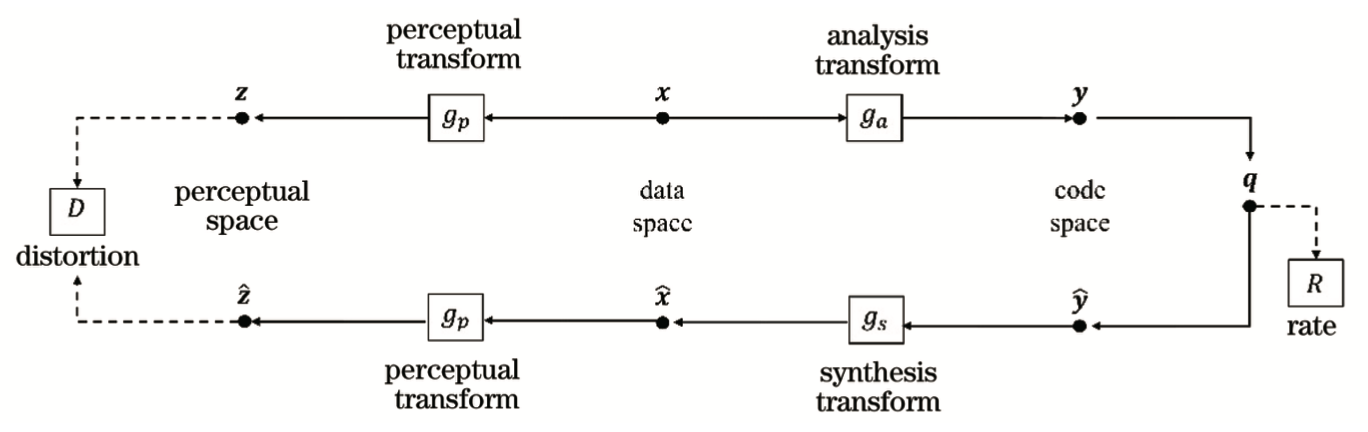
\includegraphics[width=\linewidth]{4.png}
	\caption{基于非线性变换的端到端学习图像编码框架}
	\label{fig:fig4}
\end{figure*}

前期应用神经网络技术的图像视频编码方法主要优化压缩框架中的编码工具,其主要思路都是 将 传 统 混 合 编 码 框 架和 混 合 视 频 编 码 框 架 (HVC) 中 的 模 块 与 神 经 网 络 相 结 合 来 提 升 性 能 , 但基于模块改进的性能提升有限且实现复杂。因此有必要采用端到端学习来实现整体性能的提升以满足日益增长的压缩需求。基于端到端学习的图像编码研究是从 Balé \cite{balle2016end, DBLP:conf/pcs/BalleLS16, balle2018variational}、Toderici \cite{toderici2015variable, toderici2017full}、Theis \cite{theis2017lossy} 等 的 研 究 开 始 的。最初的研究在端到端学习的压缩框架中引入了基于 CNN 或者 RNN 的自编码器,实现了可观压缩率下图像编码的整体优化重建。为了更好地表达图像相关性,研究者们一方面拓展研究了多种不同结构的自编码器,包括变分自编码器(VAE)、多尺度 自 编 码器 (MSAE)等 ,另 一 方 面 引 入 超 先 验 信 息 进 行 融 合 预 测 以 提 升 端 到 端 学 习 能 力 。 Ballé 等证 明了超先验模型中率失真优化可等效为最小化数据分 布 的 KL 散 度 (Kul lback-Leibler divergence), Zhou等 \cite{zhou2019end}提出了基于注意力机制的超先验自编码器。可见大多数基于端到端学习的图 像编码方法都依赖于自编码器的训练,以充分利 用空间相关性和数据统计分布,可在码率和失真 之间取得良好的平衡,并且可以针对任意失真指 标进行快速优化,拥有可媲美甚至超过现有国际 图 像 编 码 标 准 (如 JPEG、JPEG2000、HEVC Intra 等)的压缩性能。

除上述框架的创新外,神经网络技术也被拓展应用于图像编码中的变换、量化、熵编码等核心模块 以提升性能。变换从传统的线性离散余弦变换 (DCT)和小波变换逐步发展到非线性变换,如广义 分歧归一化(GDN)变换。在端到端学习框架中,变 换 等 效 为 利 用 逐 层 卷 积 来 提 取 特 征 激 活 (fmaps); 量化由标量量化逐步发展到矢量量化,实现从 round 函 数 到 现 在 流 行 的 软 量 化和 格 型 矢 量 量 化,这 样 可 在 满 足 数 据 压 缩 的 同 时 保 证 反 向 传 播 梯 度 可 导 ;熵 编 码 从 最 初 JPEG 使 用 的 Huf fman 编 码,发 展 到 基 于 超 先 验 和 递 归 近 邻 概 率 混 合 预 测的算术编码,实现编码性能的大幅提升; 此外, 损失函数从广泛使用的 L1损失和 L2损失,发展到改善收敛不稳定和局部最优解问题的交叉熵损 失以 及 改 善 图 像 主 观 质 量 的 感 知 损 失和对 抗 损 失,再 到 现 在 的 复 合 损 失 函 数。下面将主要对基于端到端学习的图像编码框架中这三个模块的研究现状及进展进行介绍,并对各模块中使用的方法进行了分析与对比。

\noindent\textbf{变换}~图像变换编码将空域图像像素转换为变换域系数,实现能量聚集的紧致表达,以达到压缩的目的。 大多数压缩方法都使用正交线性变换来降低数据的 相关性。在传统的变换方法中,最早针对信号冗余 解耦优化的线性变换可以追溯至 KL变换和主成分 分析法(PCA)。之后国际图像编码标准JPEG 和JPEG2000 分 别 使 用 的 离 散 余 弦 变 换 和 小 波 变 换 也 均为线性变换。

但是正交线性变换中线性滤波器响应的联合统计量呈现了很强的高阶依赖性,为解决此问题可联合局部非线性进行增益控制。近几年,端到端学习将非线性变换融入图像压缩框架中。其中,Balé 等 \cite{balle2016end, DBLP:conf/pcs/BalleLS16}提出了基于非线性变换编码的端到端学习框架,如\textbf{图\ref{fig:fig4}}所示,将图像强度向量x 先通过分析变换$y= g_a(x;\phi)$(其中 $\phi$ 为学习参数向量)映射到编码域, 再通过量化处理得到离散值向量 $q$,之后进行熵编码,相对应地,由离散值向量 $q$ 估计连续值向量 $\hat{y}$,应 用 生 成 变 换 $\hat{x}=g_s(\hat{y};\theta)$ ( 其 中 $\theta$ 为 学 习 参 数 向 量),并进行像素重建;编码决策通过率失真优化性能 ,常 见 的 失 真 度 量 包 括 均 方 误 差 (MSE)和 SSIM ,也可引入感知失真等进行性能优化,最后端到端学 习系统通过优化学习参数向量 $\phi$ 和 $\theta$ 来最小化码 率$R$和失真$D$的加权和 $R+\lambda D$ ,其中,$\lambda$控制码率 和失真的平衡。分析变换分为三个阶段:卷积、下采 样和 GDN 变换,作为其逆变换的生成变换也分为 三个阶段:仿射卷积、上采样和 GDN 逆(IGDN)变 换,且两类变换中的上下采样操作均可通过卷积来 实现,从而提高了计算效率。感知变换中归一化拉 普拉斯金字塔模型(NLP)与 GDN 的组合考虑了图像局部亮度和对比度的误差,相较于采用MSE 优化 DCT 的传统方法而言,在相似重建质量的情况下,降低了码率。

现今,自编码器被越来越广泛地用于图像压缩 中。这些研究利用单个自编码器或循环自编码器在 瓶颈层生成fmaps,用于后续的量化和熵编码 \cite{liu2018deep}。 典型的自编码器结构包含三个部分:编码器、表示压 缩数据的瓶颈和解码器,将这三个部分级联并进行 端到端训练。由于传统JPEG 等算法中线性变换对 空间相关性和压缩数据分布的利用不够充分,使用 深度卷积神经网络可实现非线性变换,对图像分布 进行更好的冗余解耦,实现更紧致的特征表达并实 现更好的压缩 \cite{theis2017lossy, zhao2018multiple, zhao2019learning, li2018learning}。

传统自编码器结构复杂、时间复杂度高,受 Shi 等 \cite{shi2016real}的工作启发,Theis等 \cite{theis2017lossy}提出基于卷积神经网 络的压缩式自编码器(CAE),对图像先进行卷积以 提取特征再进行上采样,并在解码器中采用了子像 素结构,该方法适用于高分辨率图像压缩并可大幅 度提升计算效率。对于图像编解码而言,可以通过 级联多个卷积神经网络进行定义分析和生成变换, 并允许以端到端学习的方式联合优化非线性的编码 器和解码器。因此绝大多数研究都采用了不同的卷 积神经网络进行非线性变换的设计,如 Zhao等 \cite{zhao2019learning} 利用由 CNN 组成的特征描述神经网络(FDNN)在 低维空间对真实图像(ground-truthimage)进行有 效的描述以大幅减少图像所包含的数据量,Li等 \cite{li2018learning} 用多个卷积层定义了非线性分析变换。 

综上,基于端到端学习的图像编码框架中的变 换方法从先前的正交线性变换发展到非线性变换。 现有的图像变换编码的主要作用在于提取特征以进 行更紧致的表达,且使用深度卷积神经网络的自编 码器是如今变换编码的主流方法

\noindent\textbf{量化}~在传统的图像压缩框架中,量化参数与图像质 量和码率(压缩率)息息相关。而在端到端学习的图 像压缩框架中,量化将变换后的特征激活值由浮点 数转换为规则定点数,作为后续熵编码的输入。最 常用的规则量化方法是取整函数———round函数。

由于目标失真函数主要使用梯度下降法优化端 到端编码中的率失真,反向传播中要求量化函数全 局可导,所以基于端到端学习的图像压缩研究一 直围绕着解决量化的不可导问题(量化不连续,其导 数在 任 何 地 方 都 为 零 或 无 穷 大)而 展 开。Ballé 等 \cite{balle2016end, DBLP:conf/pcs/BalleLS16}使用加性均匀噪声源代替了标量量化器实现 全局可导。

\begin{equation}
\begin{gathered}
\hat{\boldsymbol{y}}_i=\boldsymbol{q}_i=\operatorname{round}\left(\boldsymbol{y}_i\right), \\
P_{q_i}(n)=\left(p_{y_i} * \operatorname{rect}\right), n \in \mathbf{Z},\\
\widetilde{y}_i=\boldsymbol{y}_i+\Delta \boldsymbol{y}_i, \\
p_{\widetilde{y}_i}=p_{y_i} * \operatorname{rect}=\int_{n-\frac{1}{2}}^{n+\frac{1}{2}} p_{y_i}(t) \mathrm{d} t, n \in \mathbf{Z}, \\
p_{y_i}(n)=P_{q_i}(n), n \in \mathbf{Z},
\end{gathered}
\end{equation}

式中: $i$ 为索引, 遍历向量中的所有元素; $\boldsymbol{y}_i$ 为图片强 度向量 $\boldsymbol{x}_i$ 经过分析变换后的结果; $\hat{\boldsymbol{y}}_i$ 和 $\boldsymbol{q}_i$ 为 $\boldsymbol{y}_i$ 经 过量化后得到的向量; $n$ 指第 $n$ 个量化区间; $P_{q_i}$ 为 $\boldsymbol{q}_i$ 的概率质量函数; $p_{y_i}$ 为 $\boldsymbol{y}_i$ 的密度; * 代表连续卷 积; rect 为 $\left[-\frac{1}{2}, \frac{1}{2}\right]$ 的均匀分布; $\Delta \boldsymbol{y}_i$ 为均匀噪声 源, 即 rect; $\tilde{\boldsymbol{y}}_i$ 为加上均匀噪声后的 $\boldsymbol{y}_i$ 。

采用取整函数的量化将浮点数转换为整数,会 显著地降低重建的图像质量,因此 Agustsson等 \cite{agustsson2017soft} 在图像压缩的背景下探讨了矢量量化,提出软到硬 (soft-to-hard)的量化方法,让网络结合权重学习量 化级,将其应用于更广泛的问题中,并证明了矢量量 化比标量量化更具优势。传统的矢量量化需要占据 大量的存储空间且需要进行复杂的近邻搜索,对编 码器复杂度要求过高,因此 Zhao等 \cite{zhao2018multiple}提出多描述 格型矢量量化,应用对称结构避免了复杂的邻搜索。 由此可知,为解决量化的不可导问题,最常见的 方法是随机近似和用光滑导数近似的round方法。 如今矢量量化相较于标量量化成为更具竞争力的量 化方法,提出的软矢量和格型矢量的量化方法可在 保证重建质量的同时又使模型具有可微性。

\noindent\textbf{熵编码}~熵编码通过减少统计冗余进一步提升图像压缩 率。早期的深度熵编码算法能够使压缩性能得到一 定的提升,但在基于端到端学习的超先验模型出现 后,熵编码能够提供的压缩性能愈来愈高。

常用的 熵 编 码 大 多 是 变 长 编 码(VLC),其 中 包括 Huffman编码和算术编码 \cite{rissanen1981universal}。就现有的国际 图像编码标准而言,除使用 Huffman编码的JPEG 以外,其余的国际图像标准都选择使用算术编码, 目前算术编码因其可以在一个定义良好的上下文 中表现出更高的压缩率且能将量化后的fmaps转 化为 码 流 的 优 点,已 成 为 更 具 竞 争 力 的 熵 编 码 选择。

基于端到端学习的图像压缩的重要组成部分之 一是用于隐式表达的可训练熵模型,因为隐式表达 的实际分布是未知的,熵模型提供了通过近似分布 来估计编码隐式表达所需比特的方法,从而显著提 高了基于神经网络的图像压缩性能 \cite{lee2018context}。熵模型是 由 Ballé等 \cite{balle2016end}和 Theis等 \cite{theis2017lossy}首次提出的,他们的工 作对之后的研究做出了极大的贡献。前者认为隐式 表达的熵模型为非参数模型,而后者采用 GSM 模 型,其共同点在于尽可能地学习统计分布。为减少 先验和边缘信息的不匹配,Ballé等 \cite{balle2018variational}在先前研究 的基础上,通过在隐式表达的局部尺度参数上引入 超先验来捕获空间依赖性,得到更好的模型匹配,从 而增强熵模型、提升压缩性能。他们根据输入自适 应估计表达尺度,并使用 GSM 的方法将压缩的超 先验作为辅助信息添加到生成的码流中,从而允许 解码器使用条件熵模型。同年,受概率生成模型的 启发,Minnen等 \cite{minnen2018joint}提出了包含超先验和递归近邻 概率融合的自编码器,如图4所示,以两种方式扩展 了基于 GSM 的熵模型:一是将 GSM 模型推广至 GMM,在不增加模型复杂度的情况下呈现出更好 的率失真性能;二是将递归模型与超先验模型相结合。这两种结构可以互补,从而更好地利用隐式表 达的概率结构。近期,Oktay等 \cite{oktay2019scalable}又提出了一种基 于端到端学习的神经网络权值的压缩方法,该方法 先在隐式空间进行重参数化,在训练过程中采用概 率模型对参数表示施加熵惩罚,完成训练后使用 算术编码压缩隐式表达。

\begin{figure*}[!ht]
	\centering
	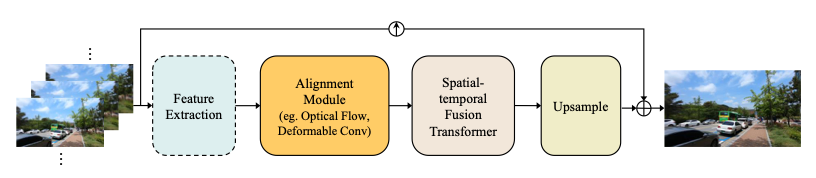
\includegraphics[width=\linewidth]{6.png}
	\caption{低比特率下 PO-ELIC 和 HiFiC 的可视化结果}
	\label{fig:fig6}
\end{figure*}

\begin{figure}[!ht]
	\centering
	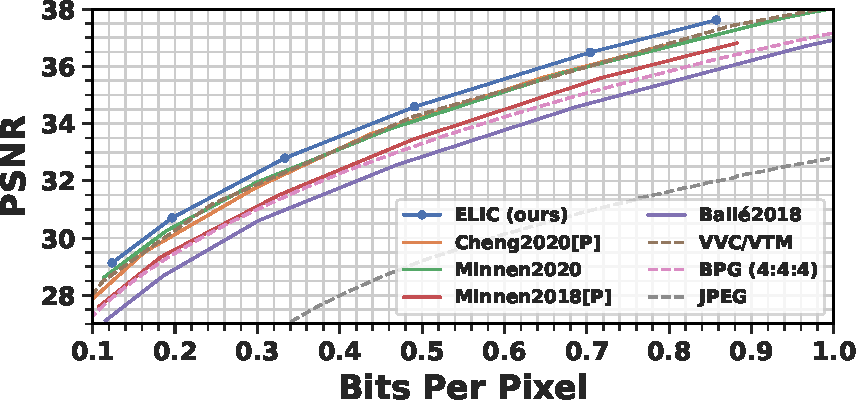
\includegraphics[width=\linewidth]{5-1.pdf}
	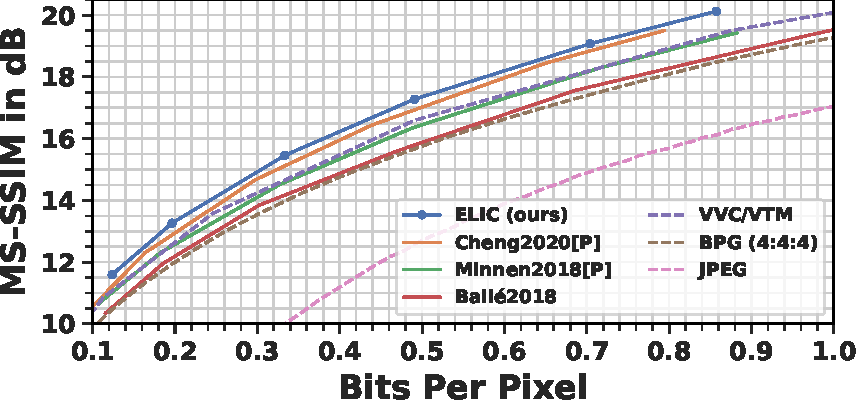
\includegraphics[width=\linewidth]{5-2.pdf}
	\caption{图像压缩方法的率失真曲线}
	\label{fig:fig5}
\end{figure}


在 Ballé等的研究基础上,Lee等 \cite{lee2018context}发现压缩 性能在本质上是取决于熵模型的容量的,因此为扩 大熵模型的容量,提出了一种上下文自适应熵模型 的框架,根据是否需要额外的比特分配,使用两种类 型的上下文:比特消耗上下文和无比特消耗上下文。 通过使用以上熵模型来更准确地估计每个隐式表达 的分布,从而更有效地减少相邻隐式表达之间的空 间依赖性,达到提高性能的目的,该研究实现的图像 压缩 性 能 在 PSNR 和 多 尺 度 结 构 相 似 性 (MS- SSIM)方面优于图像压缩的国际标准 BPG。

 综上所述,传统图像压缩框架的熵编码基本都 是 Huffman编码和算术编码,后者相较于前者而言 能够准确地呈现概率分布,更能逼近香农提出的理 论熵值。随着超先验的加入,结合了神经网络和算 术编码的混合熵模型因为有着能够近似分布、估计 编码隐式表达所需的比特以及克服隐式表达分布未 知的问题这几个优势,因此被广泛应用于基于端到 端学习的图像编码框架中。

与传统的图像编码技术相比,深度学习在训练 的阶段因其需要大量的数据量而呈现巨大的计算量 和较高的时间复杂度。而现有的应用(如云计算)可 以进行并行化,采用多 GPU 可实现数据和模型的 并行,加速深度学习的训练。训练好的模型复杂度 相对较低,硬件技术的发展和高效深度学习架构的 设计 \cite{chen2019eyeriss}有望实现实时图像编解码。同时,如今众多 的移动设备,如华为 Mate30、苹果iPhone都已经全 面支持深度学习模块,极大地促进了基于学习的图 像编解码的实际应用。除运算量这一评价指标外, 图像质量是如今图像编码研究中的主要评价指标。但无论是从数据指标还是图像质量而言,深度学习的方法均超过了传统方法。如 \textbf{图 \ref{fig:fig5}} 所示, ELIC \cite{he2022elic} 将非均匀分组模型与已有的上下文模型相结合,在不影响运行速度的情况下提高了编码性能,达到了最先进的速度-压缩率联合表现。PO-ELIC \cite{he2022po} 可以在更低的比特率下取得和 HiFiC \cite{mentzer2020high} 相当的主观感知质量,其可视化对比结果如 \textbf{\ref{fig:fig6}} 所示。

基于端到端学习的图像编码的研究只有短短几 年的历史,尽管已经取得卓越性能,但仍有较多环节 需进一步改进和完善:1)在网络结构方面,应进一步 探索新的神经网络模型在图像编码上的应用效果, 如InceptionNet、可 变 性 卷 积 等;2)在 码 率 分 配 方 面,可进一步根据图像内容差异性、特征图的分布 等,研究自适应的码率分配,以保证将码率更多地分 配在对视觉质量影响大的信息上;3)在性能方面,目 前的研究更注重压缩比和重建质量的提升,忽略了 对计算复杂度的研究和优化,但在实际应用中复杂 度是不可忽略的性能指标,因此,不仅需要研究深度 学习方法复杂度的客观衡量标准,还应以此为指导, 简化网络,实现更高效的计算;4)在硬件加速方面, 应充分考虑硬件实现的需求,对网络进行改造,从而 为将来的图像压缩芯片提供基础;5)在应用方面,随 着智能化需求的增加,图像更多地被应用于计算机 视觉,因此,可以研究图像压缩和计算机视觉之间的 共通特性,探索更有利于计算机理解和识别的图像 压缩方法。

